\documentclass{llncs}
\usepackage[none]{hyphenat}
\usepackage{graphicx}
\usepackage{url}
\sloppy

\title{Supercomputing Centers and Electricity Service Providers: A Geographically Distributed Perspective on Demand Management in Europe and the United States}
\author{Tapasya Patki\inst{1} \and Natalie Bates\inst{2} \and Girish Ghatikar\inst{3} \and Anders Clausen\inst{4} \and Sonja Klingert\inst{5} \and Ghaleb Abdulla\inst{1} \and Mehdi Sheikhalishahi\inst{6}}
\institute{Lawrence Livermore National Laboratory \and Energy Efficient High Performance Computing Working Group \and GreenLots and Lawrence Berkeley National Laboratory \and University of Southern Denmark \and The University of Mannheim \and Create-Net \\ Contact Email: patki1@llnl.gov}

%\author{Natalie Bates and Tapasya Patki \\ Demand Response Team, Energy-Efficient HPC Working Group}
%\date{\today}
%
%\setlength{\topmargin}{-15mm}
%\setlength{\textwidth}{6.5in}
%\setlength{\oddsidemargin}{0mm}
%\setlength{\textheight}{8.5in}
%\setlength{\footskip}{1.5in}

\begin{document}
%\fontsize{10}{15}
%\selectfont
\maketitle

\abstract{
Supercomputing Centers (SCs) have high and variable power demands, which increase the challenges of the Electricity Service Providers (ESPs) with regards to efficient electricity distribution and reliable grid operation. High penetration of renewable energy generation further exacerbates this problem. In order to develop a symbiotic relationship between the SCs and their ESPs and to support effective power management at all levels, it is critical to understand and analyze how the existing relationships were formed and how these are expected to evolve. \\
In this paper, we first present results from a detailed, quantitative survey-based analysis and compare the perspectives of the European grid and SCs to the ones of the United States (US). We then show that contrary to the expectation, SCs in the US are more open toward cooperating and developing demand-management strategies with their ESPs. In order to validate this result and to enable a thorough comparative study, we also conduct a qualitative analysis by interviewing three large-scale, geographically-distributed sites: Oak Ridge National Laboratory (ORNL), Lawrence Livermore National Laboratory (LLNL), and the Leibniz Supercomputing Center (LRZ). We conclude that perspectives on demand management are dependent on the electricity market and pricing in the geographical region and on the degree of control that a particular SC has in terms of power-purchase negotiation.}

\newpage

\section{Introduction}

Current Supercomputing Centers (SCs) for High-Performance Computing (HPC) with peta-scale capabilities have high power demands, with peak requirements of over 30 MW and fluctuations of a few megawatts. This trend is expected to continue in the future as we push the limits of supercomputing further. As a result, Electricity Service Providers (ESPs) for such SCs need to support efficient electricity generation, transmission and distribution along with reliable grid operation. ESPs today already face the challenge of supporting and accommodating  the megawatt-level fluctuations from SCs and often require HPC client sites to forecast their electricity use. The acceptance and proliferation of renewable sources of energy further adds to the variability at the electricity generation end, making grid reliability even more challenging. A tighter integration and open communication between ESPs and their client SCs is thus critical as we proceed toward the next generation of supercomputing. \\

At present, most ESP-SC relationships are linear and unidirectional. Power is typically generated, distributed and delivered to customer sites without direct active involvement, and most electricity pricing contracts are negotiated without tight integration requirements. Going forward, however, it is expected that a multi-directional relationship will evolve between the ESPs and SCs.  Communication and control will flow from end-customers to one or more of the electricity generation and distribution entities, and contract terms will enforce stringent usage requirements. The cloud and data center providers, such as Google, have already started to anticipate this multi-directional relationship and are taking advantage of this changing landscape.  For example, Google's response suggests vertical integration, especially with Google's Energy Subsidiary which gives Google the right to sell energy within the United States. (need citation). Another example is the SmartGrid initiative \cite{SmartGrid} by the U.S. Department of Energy, which is making electricity delivery faster and more efficient by involving customers, adjusting to dynamic demands, and by providing automated solutions and quick responses to remote locations. Techniques involved in establishing such multi-directional relationships are referred to as \emph{demand management} (DM) techniques. The Energy-Efficient High-Performance Computing Working Group (EE HPC WG) seeks to analyze the impact of similar DM techniques for SCs with HPC workloads and their ESPs. \\

In our previous work, we focused on understanding how ESPs and SCs can work together to improve energy efficiency by surveying large-scale SCs in the United States \cite{BatesESP}. We developed a questionnaire and noted that none of the SCs are working directly with their ESPs. Our main conclusion from this work was that SCs in the United States were interested in a tighter integration with their ESPs, but a business case for the same had not been demonstrated. In this work, we expand our analysis to include European SCs, where electricity is more expensive and is subject to more variability because of the use of renewable sources of energy. We expected that the European SCs would be more tightly integrated with their ESPs because of the higher prices and more extensive use of renewables in Europe.  Contrary to our expectations, however, we found that the United States shows more interest in responding to requests from their ESPs than Europe.  There are four 10+MW SCs in the United States, whereas all of the remaining SCs in both the United States and Europe are 5MW or less.  These four 10+MW SCs have all had communication with their ESPs about responding to grid requests.  Perhaps they are harbingers for the lower power demand SCs.  Another factor explaining the difference may be greater availability of electricity demand response incentive programs in the United States than in Europe. In future studies, we hope to better understand the European ESPs and their environment to see if this hypothesis has merit. 

An example of this can be seen in Figure \ref{fig:seq}, which depicts the fluctuations in megawatts on the world's third fastest supercomputer, Sequoia, which delivers 16.3 petaflops and is hosted at Lawrence Livermore National Laboratory.

%There is a movement away from a linear, uni-directional system where power is generated, distributed and delivered to customers without their involvement.  The evolving system is multi-directional (or at least bi-directional) with communication and control going from end-customers to one or more of the electricity generation and distribution entities.  The cloud providers, like Google, have already started to anticipate and take advantage of this changing landscape.  Google's response suggests vertical integration, especially with Google's Energy Subsidiary which gives Google the right to sell energy within the United States.  It is thus critical to understand the relationship between SCs and their associated Electricity Service Providers (ESPs) and to encourage the development of a more symbiotic association between the two. More specifically, it is important to analyze the expectations of SCs and ESPs from each other, and to study the willingness and feasibility of grid integration techniques. For example, the SmartGrid initiative \cite{SmartGrid} by the U.S. Department of Energy is making electricity delivery more fast and efficient by involving customers, adjusting to dynamic demands, and providing automated solutions and quick responses to remote locations. T
\begin{figure}
\begin{center}
\frame{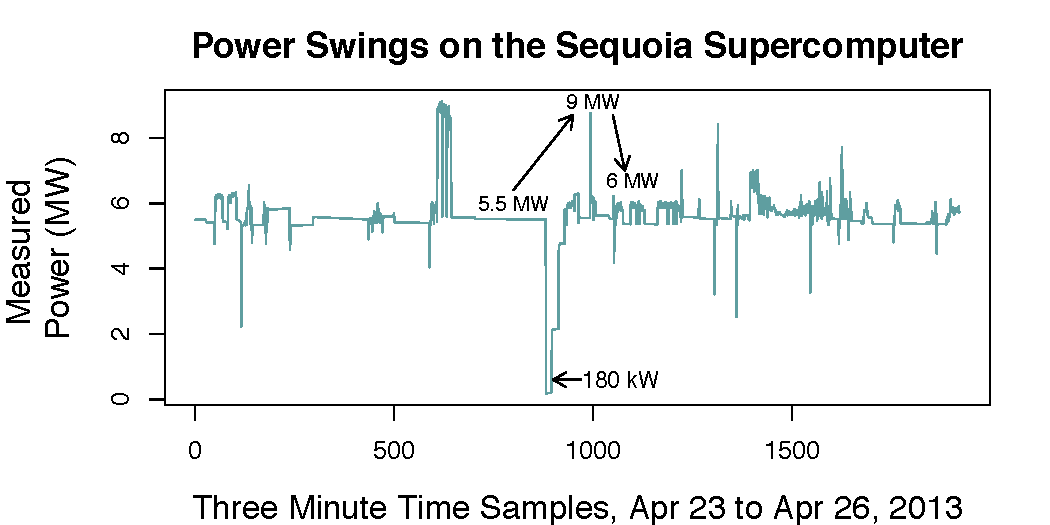
\includegraphics[scale=0.6]{figs/seq.pdf}}
\caption{Sequoia Supercomputer Power Swings}
\label{fig:seq}
\end{center}
\end{figure}



We accomplished expanding our analysis to Europe by extending the aforementioned questionnaire to European SCs. Nine out of the sixteen SCs that we contacted responded to the questionnaire. All except one of these sites were in Top 50 supercomputers in the world \cite{Top500}. Section \ref{res} presents an overview of our results from the questionnaire. Section \ref{spm} discusses the strategies, programs and methods that were used in the questionnaire and the willingness of respondents to consider these options. Section \ref{comm} highlights some of the comments we received from our respondents, and Section \ref{summary} concludes this article.

\section{Motivation for Demand Management}
\label{strategies}
We measured the power consumption of Sequoia, the world's third fastest supercomputer at 17.1 petaflops, hosted at LLNL. Sequoia is a BlueGene/Q design-based system with 98,304 16-core PowerPC A2 compute nodes that has a power rating of 7.9 MW. The data from Sequoia was collected at three-minute intervals over three days and the results can be seen from figure \ref{fig:seq}. Information about the workload being executed was not made available. The y-axis is the power consumed, and the x-axis represents the time samples.  As can be noted from this figure, fluctuations of a few megawatts are fairly common. Some of these fluctuations may be related to maintenance cycles and could be scheduled or forecasted. However, there are other times where the fluctuations are not scheduled in advance and may occur as a result of the workload that is executing on the supercomputer. \\

\begin{figure}
\begin{center}
\frame{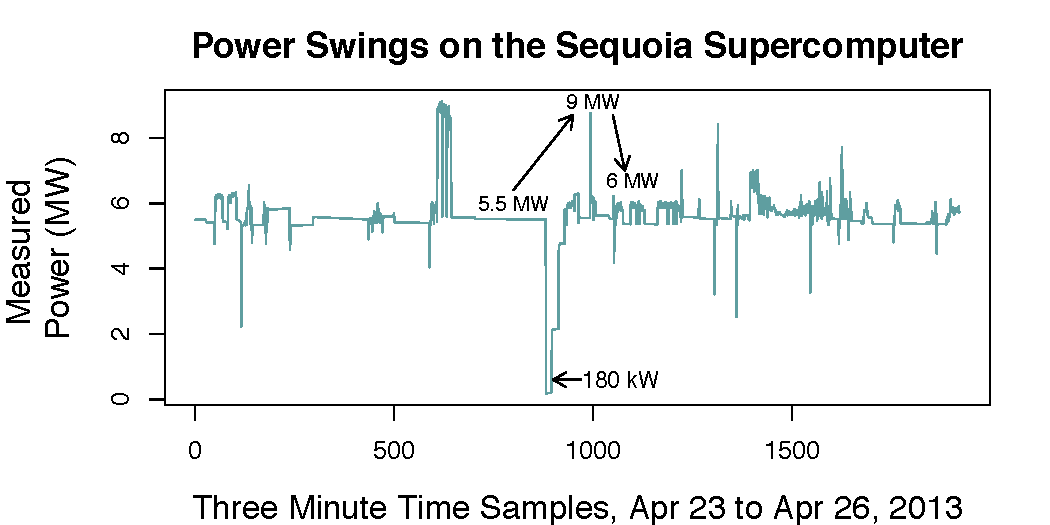
\includegraphics[scale=0.6]{figs/seq.pdf}}
\caption{Sequoia Supercomputer Power Swings}
\label{fig:seq}
\end{center}
\end{figure}

\begin{figure}
\begin{center}
\frame{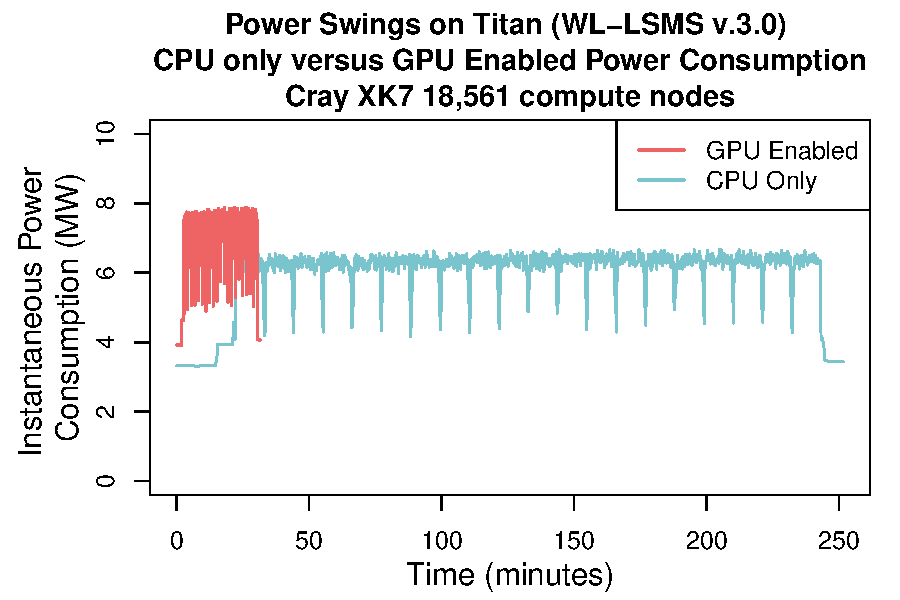
\includegraphics[scale=0.6]{figs/ORNLData.pdf}}
\caption{Titan Supercomputer Power Swings}
\label{fig:titan}
\end{center}
\end{figure}

We observe similar trends with data from Titan, which is the world's second-fastest supercomputer and is hosted at ORNL. Titan is a 17.6 petaflop system with a power rating of 8.2 MW. It comprises of 18,688 16-core AMD Opteron 6274 compute nodes, and each compute node has a NVIDIA Tesla K20X GPU. Figure \ref{fig:titan} shows data gathered from a identical WL-LSMS executions on the Titan supercomputer. WL-LSMS is a benchmark that performs thermodynamic calculations  \cite{WLLSMS}. The graph in Figure \ref{fig:titan} has instantaneous power in MW on the y-axis and the benchmark execution time on the x-axis. The data is reported for a CPU-only run as well as a GPU-enabled run. The power samples for the CPU-only run were collected every 8 minutes, where as the samples for the GPU-enabled run were reported every second. The red line represents the GPU-enabled run and the blue line represents the CPU-only run.  As can be noted from this data, huge power swings are observed on Titan, both in the case of CPU-only as well as GPU-enabled runs. 
The energy efficiency improves by about seven times when the GPU is enabled as the application runs significantly faster. However, note that the peak power and power fluctuations are greater with the GPU-enabled run than they are with the CPU-only run.  Peak power increased by more than one megawatt and power variability increased by more than one half megawatt. 

This behavior can be attributed to the fact that the GPU has very sophisticated power management features and is ready to go in an instant, ramping up both operational frequency and power. However, when it is idle, it almost powers itself down.  Regardless of the cause, the net effect is that less energy is used to get the same work done in the GPU-enabled case., but with higher power draw and greater power variability.

Both these datasets clearly indicate that huge power fluctuations occur in real production systems, and this can affect the reliability of the ESP grid. It is thus imperative to understand how such variable power demands can be managed better, and how SCs can forecast and communicate with their ESPs more often to discuss and address such issues. 

\subsection{Techniques for Demand Management}
We now explain different approaches used in demand management by SCs. We define \emph{strategies} as power management techniques used by SCs to manage power and provide load flexibility. Strategies may or may not improve energy efficiency. For example, \emph{Load Migration} is a strategy that SCs may use in response to an ESP's request, and while it helps manage power effectively, it does not impact the energy efficiency of the site. On the other hand, \emph{fine-grained power management} techniques, such as using node-level power capping, or better job scheduling algorithms are likely to improve energy efficiency but may not be as useful in response to an ESP request. Almost all sites employ some power management strategies, especially the ones involving lighting, temperature, cooling, fine-grain power management and job scheduling. 

\emph{Programs} are incentives offered by ESPs to their customers and to SCs in order to motivate them to help balance the electrical grid and perform power managment. Common examples include peak shedding, peak shifting and dynamic pricing. Peak shedding describes the action where SCs (or consumers) reduce their electricity consumption in response to a request from the ESP. The reduction in electricity consumption does not lead to an increase in consumption at a later point in time. Peak shifting, on the other hand, moves load from one time slot to another, in response to a request from the ESP. Lastly, dynamic pricing is a mechanism used by the ESP to incentivize an increase or decrease in consumption by varying the price of electricity over time.

\emph{Methods} are used by the ESPs to balance the electrical grid in the transmission and distribution phases. Examples of methods include regulation, frequency response, grid scale storage and use of renewable sources of energy. 
\section{Quantitative Study: Europe and United States}
\label{res}
In this section, we discuss the results from our quantitative survey. We extended our questionnaire from our previous work \cite{BatesESP} and contacted sixteen SCs in the European region.  Appendix \ref{appendixA} provides an overview of the questionnaire. The detailed definitions for each of the demand management approaches and strategies can be found in our previous work \cite{BatesESP}. Nine out of the sixteen European SCs that we contacted responded to the questionnaire. All except one of these sites were in Top 50 supercomputers in the world \cite{Top500}. 


\begin{figure}[ht!]
\begin{center}
\frame{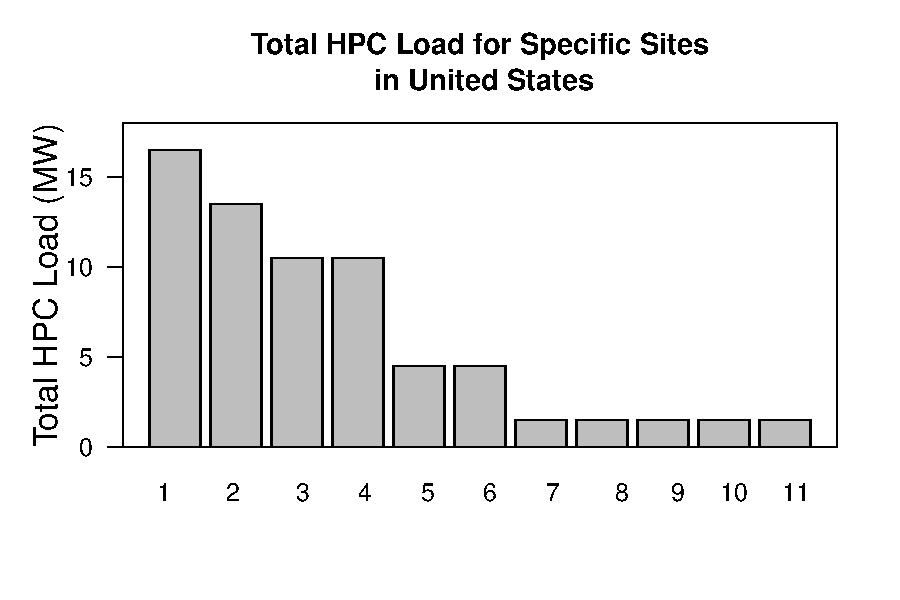
\includegraphics[scale=0.58]{figs/loadgraphUS.pdf}}
\caption{Total Load at at SCs in United States}
\label{fig:USload}
\vspace{0.9cm}
\frame{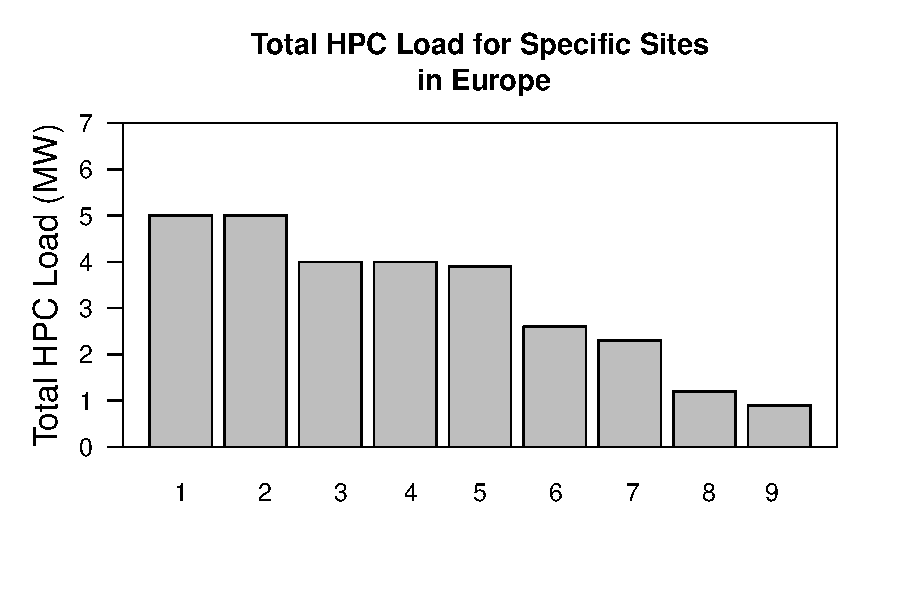
\includegraphics[scale=0.58]{figs/loadgraphEU.pdf}}
\caption{Total Load at at SCs in Europe}
\label{fig:EUload}
\end{center}
\end{figure}

Figures \ref{fig:USload} and \ref{fig:EUload} depict the total load in megawatts for each of the respondents in the United States and in Europe. Most supercomputing sites have a total load of under 5 MW (sixteen out of twenty). Four of the surveyed supercomputing sites had a total load of over 10 MW. 

\begin{figure}[ht!]
\begin{center}
\frame{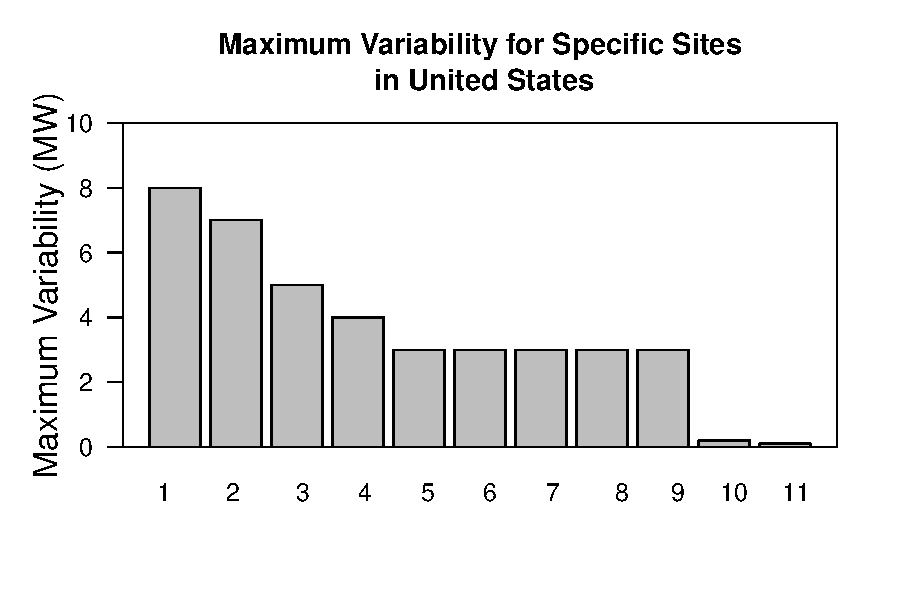
\includegraphics[scale=0.58]{figs/vargraphUS.pdf}}
\caption{Maximum Variability at at SCs in United States}
\label{fig:USvar}
\vspace{0.9cm}
\frame{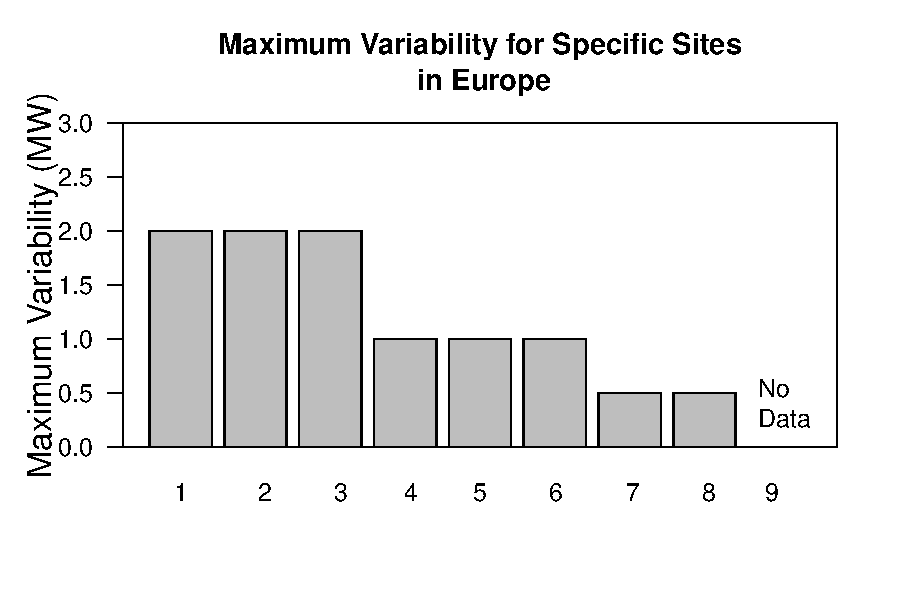
\includegraphics[scale=0.58]{figs/vargraphEU.pdf}}
\caption{Maximum Variability at at SCs in Europe}
\label{fig:EUvar}
\end{center}
\end{figure}

Both United States and Europe had power swings and fluctuations of a few megawatts. In our questionnaire, we asked respondents to report the maximum variability that they have experienced in their SCs. The results of these for United States as well as Europe are shown in Figures \ref{fig:USvar} and \ref{fig:EUvar} respectively. In the United States, three of the eleven sites surveyed had maximum variability of over 5 MW. For our United States respondents, the minimal option for reporting this was ``Less than 3 MW'', because of which we could not capture less intense power swings. In the European survey, we allowed the respondents to provide a more accurate value, and as shown in Figure \ref{fig:EUvar}, we observed power swings in the range of half a megawatt to about 2 MW. Almost all of the respondents reported that this variability is due to maintenance cycles, and that it can be scheduled \emph{day-ahead} if necessary.

In terms of demand management strategies, the survey indicated that there is moderate interest in grid integration strategies such as coarse- and fine- grained power management or temperature control in the United States, and low interest for the same in Europe. From the point of view of SCs, strategies such as cutting jobs or load migration have little or no interest. 

From our questionnaire, we also concluded that neither European nor the United States sites are engaged with peak shedding, peak shifting or dynamic pricing programs at present. More sites in the United States have communicated with their ESPs regarding these programs. While both European and United States SCs are interested in dynamic pricing, there is mixed interest in peak shedding and peak shifting. The European sites are more interested in peak shedding than peak shifting, but the United States sites are more interested in peak shifting. Both European and US sites are interested in discussing renewables with their ESPs, but there is little interest in communicating with regards to the other possible methods.

\begin{table}[h]
\begin{center}
\begin{tabular}{|l|c|c|c|c|}
\hline
\multicolumn{5}{|p{.72\textwidth}|}{\emph{Ques:} Please evaluate as high, medium or low the following motivations for your site's interest in pursuing a stronger relationship with your electricity service provider}\\
\hline
& Low & Medium & High & Rating Count \\
\hline
Economically justified & 14.3\% (1) & 28.6\% (2) & 57.1\% (4) & 7 \\
\hline
Good citizen & 14.3\% (1) & 71.4\% (5) & 14.3\% (1) & 7 \\
\hline
Adverse consequences & 66.7\% (4) & 16.7\% (1) & 16.7\% (1) & 6 \\
\hline
Government regulation & 71.4\% (5) & 28.6\% (2) & 0.0\% (0) & 7 \\
\hline
\end{tabular}
\end{center}
\caption{Motivation for communicating with ESP (European Respondents)}
\label{fig:table2}
\end{table}

We also asked our European respondents to indicate what might motivate them to communicate with their ESPs. The results are shown in Table \ref{fig:table2}. As can be noted from this table, the main motivators are the financial incentives and the desire to be ``good citizens.'' Thus, SC motivations are driven by market-based mechanisms that justify economics and social-responsibility, even under the absence of regulatory support.

\begin{table}[h]
\begin{center}
\begin{tabular}{|p{0.265\linewidth}|p{0.265\linewidth}|p{0.265\linewidth}|}
\hline
\textbf{Program} & \textbf{Europe} & \textbf{United States}\\
\hline
Peak Shedding & 1 & 6\\
\hline
Peak Shifting & 0 & 4\\
\hline
Dynamic Pricing & 0 & 5\\
\hline
\end{tabular}
\end{center}
\caption{Communications with ESPs regarding available programs}
\label{fig:table3}
\end{table}
We noted that none of the European SCs communicated about grid integration potential, demand management and available flexibility with their associated ESPs. Additionally, there was little interest in a tighter integration with the ESPs. In general, the SCs in the United States seem to have a closer relationship with their ESPs than the ones in Europe. This can also be verified from Table \ref{fig:table3}, which shows that only 1 of the 9 respondents in Europe have had a discussion with their ESP. 

\subsection{Comments from Survey Respondents}
\label{comm}
From the comments section in our questionnaire, we noted that all SCs are already using \emph{demand forecasting} to communicate their upcoming demands and maintenance cycle schedules with their ESPs. For example, one comment was ``We project hourly average power at least a day in advance, within +/- 1MW''. Another interesting comment was ``We've to ensure that our power load neither over- nor under-shoots the contracted power band. In any cases of foreseen power abnormalities we've to inform our grid provider at least two days ahead of schedule.''

One of the SCs mentioned that they could not provide the forecast that was being asked by their ESP. More specifically, their comment indicated that their ESP asked for ``multi-year forecast of energy requirements, additional detailed forecasting and ultimately real time data, and power projections, hour by hour, for at least a day in advance.''

When it came to ESP programs, the United States SCs showed more interest. ``Our site generates 30-35 MW of power yet still imports 5-10 MW. As a large generation source the utility providers see the campus as a highly attractive partner for offloading grid stress. automatic load shedding is being explored/deployed today,'' one of the SCs noted. Another comment was ``[We are] working on load sharing of data with utility to provide better scheduling tools and address potential grid changes.'' One of the SCs mentioned that they demonstrated that peak shedding and shifting was possible, but not deployed due to its impact on HPC productivity. 

The European SCs, on the other hand, did not have much knowledge about ESP programs. Some of the responses were ``There are not so many related options and features offered by providers. We are open to further and pro-active efforts as long as providers have other kinds of programs to propose'' and ``With many of your questions I am wondering about the kind of contracts other centers might have and about the quality of some electricity providers.''

The comments also indicated that the SCs in United States are investigating the impact of power fluctuations on the electrical grid. ``[We are] working directly with provider to ensure that the effects of large load swings are understood. Have funded a simulation that accounts for all loads.'' and ``Our provider has no problem with our load swings. They indicate no concern with our next system either, but we are still looking into possible options in case there actually is a problem.'' were some of the interesting responses.

\section{Qualitative Analysis: Site-Specific Interviews}
\label{intws}

The results presented in the previous section were based on data gathered through a questionnaire created for HPC centers based on experience from a United States context. The preliminary results of the comparison across the geographical regions gave the impression that European SCs had very limited communication with their ESPs with respect to grid integration. 
However, it was apparent that some SCs in Europe engage in collaboration with their ESPs in order to ensure minimal fluctuations as well as for forecasting of deviations from normal power consumption patterns. 
In order to shed light on the details of the relationships between SCs and ESPs that were not captured in the questionnaire, we designed a qualitative interview and surveyed ORNL, LLNL and LRZ. The thesis was that a qualitative analysis will yield more complete information and will enable us to present more thorough comparative study on the status of grid integration of SCs in Europe and the US. For each site, we asked the questions listed below. We present the information from each SC in the subsections that follow.

\begin{itemize}
\item {What is your responsibility for negotiating the contract between your HPC facility and your ESP? }
\item {Could you elaborate on the details of the pricing structure on your electricity? Note that for this question, we did not request specific information on the actual price the SC pays for electricity. We were mostly interested in the type of pricing program they are enrolled in.} 
\item {Do you have any obligations towards your ESP, and if so, what is your incentive towards committing to these obligations? These obligations are characterized by being static and ?pre-smart grid? in the sense that no real-time communication is needed between ESP and SC. Examples include limits for allowed variability in power consumption and/or fixed power consumption limits. Examples for potential incentives include reduction in electricity price, enabling of direct payments and legislation benefits. }
\item{Do you offer any kind of services for your ESP, and if so, what is your incentive for offering these services? These services are characterized by two way communication between the site and the ESP, where a consumer reacts to information sent by the ESP. Examples include load capping, powering up backup generations, etc.}
\item{How do you envision your future relationship with your electricity provider? (Possible answers were: tighter, for example, by selling local generation capacity; or looser, for example, by being self-sufficient with regards to electricity needs.}
\end{itemize}


%Table \ref{tabIntw} presents details of this qualitative analysis. We have recorded the results in a tabular form to facilitate comparison between the three sites under consideration. 
%
%\begin{table}
%\centering
%\label{tabIntw} 
%\begin{tabular}{|l|l|l|l|}
% \hline
% \bf{Site} & \bf{ORNL} & \bf{LLNL} & \bf{LRZ} \\ 
% \hline
% HPC System & Titan & Sequoia & SuperMUC \\ 
% \hline
% HPC workload & Basic Science & Basic and & Academic \\
% type &&Nuclear Science&\\
% \hline
% HPC workload & Low & Mission-critical & Low\\
% criticality&&&\\
% \hline
%Point of contact & Jim Rogers & Anna-Maria Bailey & Herbert Huber\\
%\hline
%Responsibility & None, contract & None, contract & None, contract \\
%in negotiating & negotiated by DOE & negotiated by DOE & negotiated at \\
%contract with&&&the site-level by\\
%ESP &&&management\\
%\hline
%Electricity &Demand as well&Only energy & Energy is very\\
%Pricing & as energy charges,&charges, flat&expensive, high power \\
%Structure & depends on season&rate, relatively&taxes as well as\\
%&and time of day. &cheap. Thus care about&season dependent.\\
%&Operate within&utilizing all &Operate within\\
%&a power band&allocated power&power band\\
%\hline
%Power cost & & & \\
%as percentage&About 25-30\%&Under 8\%&About 50\%\\
%of TCO&&&\\
%\hline
%Obligations &&&\\
%Toward ESPs &None, and&None, and&None, and\\
%(and offered & no incentive either& no incentive either&no incentive either\\
%incentives for &&&\\
% the same)&&&\\
%\hline
%Services for &None, except&None, except&None, except\\
%ESPs&maintenance or&maintenance or&maintenance or\\
%&general&general&general\\
%&forecasting&forecasting&forecasting\\
%\hline
%Future &Will use the &Will use the&Will use the \\
%relationship &same, reliable ESP&same, reliable ESP&same ESP, flexibility\\
%with ESP&&&decisions are political.\\
%\hline
% \end{tabular}
% \end{table}

\subsection{ORNL}
For ORNL, the DOE negotiates the contract with the ESP.  ORNL gets its power from TVA, which generates, transmits and distributes the power. The DOE and TVA negotiate the power capacity that is being provisioned each year. Typically, a range for operation is chosen, for the current year, this range is 35 MW to 75 MW. 
In terms of electricity pricing, ORNL incurs two kinds of charges: a demand charge, which is fixed for a month, and an energy charge based on actual power consumption. The demand charge is determined by analyzing 30 minute blocks and by determining the peak or maximum value for the month. The demand charge can be off-peak or on-peak based on the time of the day. It has a time-of-use per day component. The energy charge is a step function. The base charge for energy is under 4 cents per kwh, which is low when compared to the industry. Also, the more energy the site consumes in kWh, the lower is the base charge. As a result, ORNL wants to keep its systems fully utilized in terms of power. Including all the costs as well as seasonal charges, ORNL pays about 9.4 cents per kWh. ORNL's provider, TVA, is not affected by power swings of a few megawatts (5 to 8 MW) and is very reliable. \\

ORNL does not have any obligations and provide any services to its ESP.  The only requirement is to operate in the range that was negotiated (35 MW to 75 MW). They have a model that explains their power usage that they provide to the TVA annually, but there is no two-way communication or forecasting or In general, the capital expenditure for the supercomputing center dominates the operational costs. As the HPC system cost depreciates with time (for example, Titan's depreciation is about 20K dollars per hour), there is little financial incentive to be flexible and to save on electricity costs, as the capital expenditure dominates the operational expenditure. The goal is thus to keep their site fully utilized in terms of power. 

\subsection{LLNL}
In the case of LLNL, the DOE negotiates the contract with the ESP with the help of a consulting company called Exeter.  A bulk purchase of power is made for about 100 MW of power capacity from the California-Oregon Transmission Project or COTP and is shared between LLNL and two other DOE sites. PG\&E is used for transmission and distribution and WAPA is used for generation. In terms of electricity pricing, LLNL does not pay a demand charge, but only pays a flat energy charge of about 4.5 cents per kWh, which is on the lower side when compared to the industry. Forecasting is done on a regular basis to be a good citizen. There is no financial incentive to save energy costs. There are no obligations from the ESP and no services are provided. The goal is to keep the site fully utilized in terms of power and to minimize leftover power.  

\subsection{LRZ}
The power contract between LRZ and \emph{Stadtwerke M�nchen}, a Munich Power Company
is the result of pan-European procurement. LRZ purchases a basic power band for one
or multiple years at the European power stock exchange. Hence, the power price is
determined by the European stock market. Additionally, there are charges for the
power grid, renewable energy, concession levy as well as taxes which are significant.
The charges for power generation and distribution constitute only 25\% of
the power price in Germany. As a result, the energy costs are very expensive for LRZ.

LRZ operates in a 4 to 6 MW power band. Typically, they pay about
17.8 Euro-cents per kWh. Having consistent power consumption is usually considered better,
as huge power swings result in much higher electricity costs. It is thus imperative
to be able to forecast any power swings and to inform the ESP about
the same. Better prediction models for power usage will definitely benefit
LRZ in terms of electricity costs, as one of their goals is to save on
energy costs. This is primarily because their energy costs dominate their
operational costs. Typically, LRZ lets the ESP know about 2 days in
advance for any scheduled downtimes. At present, there are no major
obligations toward or services provided to the ESP, mostly because of
the QOS guarantees that have to be adhered to for their users.

\subsection{Analysis}


\section{Related Work}
\label{relwork}
Data centers are known to be capable of providing flexibility in their power consumption, and thus are great candidates to participate energy market demand response (DR) programs. Wierman et. al.~\cite{WiermanIGCC} survey the opportunities and challenges for data center DR participation. Aikema et. al.~\cite{aikema2012data} overview multiple types of ancillary service markets, and study the capacity and potential benefit by introducing a simple data center participation model. Siano et al. \cite{siano2014demand} present a survey of DR for smart grids. Ghatikar et. al.~\cite{ghatikar2012demand} exploit various load management techniques, such as load shedding and shifting for data center DR. Goiri et. al.~\cite{goiri2015matching} propose GreenSlot, a workload scheduler to maximize the green energy consumption (that is, solar energy) while meeting the job deadline. Geographic load migration is another broadly studied data center management technique to help balance the grid, and reduce the energy cost exploiting the electricity price differences~(\cite{wangexploring,wang2013data,chiu2012electric,liu2011greening,lin2012online}). \\

The participation of data center in traditional DR programs, such as real-time dynamic energy pricing~(\cite{wang2013sequential,ghamkhari2012data,liu2014pricing}) and peak shaving~(\cite{urgaonkar2011optimal,PSUSigmetrics12,aksanli2013architecting}), has been widely studied. Recently, there are a growing number of interests on the data center participation in emerging DR programs that are more profitable. Chen et. al.~\cite{chenASPDAC} develop real-time dynamic control policies by leveraging both server level power management techniques and server state switches for data centers to provide regulation service reserves (RSRs). They also implement a prototype of the control policies on real-life server clusters with virtualized CPU resource limits~\cite{chendynamic}. Brocanelli et al.~\cite{brocanelli2013joint} propose the joint management of data center and employee Plug-in Hybrid Electric Vehicles (PHEVs) to increase the regulation profit. A systematic comparison shows that RSR is a more profitable program for data centers to participate than traditional programs such as peak shaving~\cite{chenIGCC}. Clausen et al. \cite{clausen2014load} found that smaller data centers aggregated through a Virtual Power Plant are a potential resource in demand management, but no electricity markets that aimed to facilitate this type of resource existed in Denmark. However, Energinet.dk and other Nordic transmission system operators do recognize demand response and demand-side market participation as a resource in grid management, and have set forth initiatives to reducing market barriers towards this type of capacity.





\section{Summary and Next Steps}
\label{summary}

\begin{table}[h]
\begin{center}
\begin{tabular}{|p{0.265\linewidth}|p{0.265\linewidth}|p{0.265\linewidth}|}
\hline
\textbf{Program} & \textbf{Europe} & \textbf{United States}\\
\hline
Peak Shedding & 1 & 6\\
\hline
Peak Shifting & 0 & 4\\
\hline
Dynamic Pricing & 0 & 5\\
\hline
\end{tabular}
\end{center}
\caption{Communications with ESPs regarding available programs}
\label{fig:table3}
\end{table}
In summary, we believe that the European ESP programs for DM need to be studied in greater detail, and the awareness of the benefits for these programs needs to be raised among the SCs. In general, the SCs in the United States seem to have a closer relationship with their ESPs than the ones in Europe. This can also be verified from Table \ref{fig:table3}, which shows that only 1 of the 9 respondents in Europe has had a discussion about programs with their ESP. As part of our future work, we want to explore the European ESP programs further, the lack of such closer relationships, and also conduct a similar study in Japan, which has different institutional and electricity supply challenges.

\section {Additional Authors}
Torsten Wilde, Leibniz Supercomputing Center\\
James H. Rogers, Oak Ridge National Laboratory\\
Ayse Coskun, Boston University\\
Hao Chen, Boston University\\
Peter M. Schwartz, Lawrence Berkeley National Laboratory\\
Gert Svensson, KTH Royal Institute of Technology\\
Bo Norregaard Jorgensen, University of Southern Denmark


\bibliographystyle{plain}
\bibliography{hao,refs}

\appendix
\section{Appendix}
\label{appendixA}

The details of our questionnaire are presented below. Our questions focused on the HPC load, power variability and demand management approaches. 

\begin{enumerate}
\item{What is your total facility energy? This should be the same as the total facility energy number that is used for calculating PUE.}
\item{ What is your total HPC load?}
\item{What is your facility PUE?}
\item{What is your facility's theoretical peak energy, as the infrastructure is currently fit up?}
%\item{What is the maximum \emph{unscheduled} intra-�hour variation in total facility energy that is likely to re-�occur?}
%\item{What is the maximum \emph{scheduled} intra-�hour variation in total facility energy that is likely to re-�occur?}
\item{What is the maximum intra-�hour variation in total facility energy that is likely to re-�occur?}
\item{Do you employ coarse-grained power management strategies?}
\item{Do you employ fine-grained power management strategies?}
\item{Do you employ load migration as a strategy?}
\item{Do you employ job scheduling as a strategy?}
\item{Do you employ back-up scheduling as a strategy?}
\item{Do you employ shutdown as a strategy?}
\item{Do you employ lighting control as a strategy?}
\item{Do you employ increasing air temperature as a strategy?}
\item{Do you employ liquid temperature adjustment as a strategy?}
\item{Do you cut jobs as a strategy?}
\item{Are there any other strategies that you employ to manage and control your total facility energy in response to a request from your energy utility/provider?}
\item{Please evaluate each of the above strategies from questions 7 to 16 as high, medium or low, based on the MW impact of each of these strategies as a response to a grid request.}
\item{Have you had conversations with your electricity service provider about peak shedding?}
\item{Have you had conversations with your electricity service provider about peak shifting?}
\item{Have you had conversations with your electricity service provider about dynamic pricing?}
\item{Have you had conversations with your electricity service provider about grid scale storage?}
\item{Have you had conversations with your electricity service provider about power variability related to renewables and methods used for responding to such variability?}
\item{Have you had conversations with your electricity service provider about frequency response?}
\item{Have you had conversations with your electricity service provider about regulation?}
\item{Have you had conversations with your electricity service provider about congestion?}
\item{Is there information you would like from your provider that you are not getting? If yes, please describe what you would like to know.}
\item{Is your provider asking for information from you that you are not able to provide? If yes, please describe what they are asking for.}
\item{Do you experience any power quality issues at your HPC facility? If yes, please describe.}
\item{Do you know of any consequences between your site and your provider from either scheduled or un�scheduled intra-�hour power variations?}
\item{Please evaluate as high, medium or low the following motivations for your site's interest in pursuing a stronger relationship with your electricity service provider.}
\item{ Please help us understand the economic aspects of power saving strategies. This is an open ended question and we encourage any feedback. For instance, what might it take to induce your site to participate in programs offered by your electricity service provider? What are the trade�offs between savings and loss of scientific productivity and equipment depreciation.}
\end{enumerate}



\end{document}
